\documentclass{aastex631}

\usepackage{amsthm, amsmath, amssymb}
\usepackage{latexsym,graphicx,rotating,amsmath, epsfig, natbib, graphbox}
\usepackage{listings}

\newcommand{\sol}{\odot}
\newcommand{\del}{\nabla}
\newcommand{\cross}{\times}
\newcommand{\avg}{\bar}
\renewcommand{\vec}{\boldsymbol}
\newcommand{\pomega}{\varpi}
\newcommand{\conv}{\boldsymbol}
\newcommand{\grad}{\vec{\del}}
\renewcommand{\d}{\mathrm{d}}

\newcommand{\scrD}{\mathcal{D}}
\newcommand{\scrH}{\mathcal{H}}
\newcommand{\scrR}{\mathcal{R}}
\newcommand{\scrL}{\mathcal{L}}
\newcommand{\scrS}{\mathcal{S}}
\newcommand{\scrP}{\mathcal{P}}

\newcommand{\Ma}{\mathrm{Ma}}
\newcommand{\Ra}{\mathrm{Ra}}
\newcommand{\Ek}{\mathrm{Ek}}
\renewcommand{\Pr}{\mathrm{Pr}}
\newcommand{\Pm}{\mathrm{Pm}}
\newcommand{\RoCsq}{\mathrm{Ro}_\mathrm{C}^2}
\newcommand{\RoC}{\mathrm{Ro}_\mathrm{C}}

\newcommand{\expm}{\mathrm{expm1}}

\newcommand{\dedalus}{\href{http://dedalus-project.org/}{Dedalus}}

\definecolor{codegreen}{rgb}{0,0.6,0}
\definecolor{codegray}{rgb}{0.5,0.5,0.5}
\definecolor{codepurple}{rgb}{0.58,0,0.82}
\definecolor{backcolour}{rgb}{0.95,0.95,0.92}
\definecolor{codered}{rgb}{0.6,0,0}
\definecolor{codeblue}{rgb}{0,0,0.6}

% \watermark{text}
\begin{document}


Momentum equation:

\begin{equation}
    \partial_t \vec{u} + \vec{u}.\del \vec{u} = -\Bigg[\dfrac{h_{c}\tau^{2}}{L^{2}}\Bigg] \del \Bigg(h+\dfrac{\phi_c}{h_{c}}\phi \Bigg) +  \Bigg[\dfrac{h_{c}\tau^{2}}{L^{2}}\Bigg] \Bigg[ \dfrac{s_{c}}{c_{P}} \Bigg] h \del s - \Bigg[\dfrac{\mu \tau}{\rho_{c}} \Bigg] \dfrac{1}{\rho} (\del.E_{ij} + \del ln(\mu).E_{ij})
\end{equation}


Entropy equation:

\begin{equation}
    \partial_t s + \vec{u}.\grad s = \dfrac{1}{\rho h}[c_{P}\Phi + \grad . (K \grad h) - c_{P}(\grad . F_{0}) ]
\end{equation}
\begin{equation}
    \Bigg[\dfrac{s_{c}}{c_{P}}\Bigg] (\partial_t s + \vec{u}.\grad s) = \Bigg[\dfrac{(\mu/\rho_{c}\tau)}{L^{2}} \Bigg] \Bigg[\dfrac{L^{2}}{\tau h_{c}}\Bigg] \dfrac{1}{\rho h} \Phi + \Bigg[\dfrac{\tau/(\rho_{c}c_{P})}{L^{2}} \Bigg]\dfrac{1}{\rho h} \grad.(K\grad h) + \Bigg[\dfrac{(K/(\rho_c c_{P})\tau)}{L^{2}} \Bigg] \dfrac{1}{\rho h} \epsilon
\end{equation}
Equation of state:

\begin{equation}
    \Bigg[\dfrac{s_{c}}{c_{P}} \Bigg] \gamma s = \text{ln}~h - (\gamma-1)\text{ln}~\rho
\end{equation}

Under hydrostatic balance, $\vec{u}=0, \partial_t = 0$, and $\dfrac{s_{c}}{c_{P}}=1$, the above equations reduce to:

\begin{equation}
    \del h + \dfrac{\phi_c}{h_{c}} \del \phi = h\del s
\end{equation}

\begin{equation}
    \grad.(K\grad h) = -\epsilon
\end{equation}

\begin{equation}
    \gamma s = \text{ln}~h - (\gamma-1)\text{ln}~\rho
\end{equation}

\begin{equation}
    K \del^{2}h + \grad K.\grad h = -\epsilon
\end{equation}
For Kramers' opacity, we have $K=K_{0} \dfrac{h^{3-b}}{\rho^{a+1}}$. Here, $K_{0}=\dfrac{16\sigma_{SB}}{3\kappa_{00}}$. We have, 

\begin{equation}
    \del \ln{K} = \dfrac{1}{K} \del K 
\end{equation}

\begin{equation}
    \del \ln{K} = K_{0} [(3-b)\del \ln{h} - (a+1)\del \ln{\rho} ]
\end{equation}

Using, $\theta = \ln{h}$ and $Y=\ln{\rho}$, we have a nonlinear boundary value problem to solve,

\begin{equation}
    \del h = - \del \phi+ h \del s 
\end{equation}

\begin{equation}
    (\gamma-1)Y + \gamma s = \log h
\end{equation}

\begin{equation}
 \del^{2}h = - h K_{0} \grad \theta . [(3-b)\grad \theta - (a+1)\grad Y] -\dfrac{\epsilon}{K}
\end{equation}

Here, we use the following boundary conditions,

\begin{equation}
    h(z=0) = h_{bot};~ h(z=L_{z}) = h_{top};~ Y(z=0) = 0
\end{equation}
Alternatively, we can formulate the above equations in the form of $\theta$ using,

\begin{equation}
    \dfrac{\del h}{h} = \del \theta
\end{equation}
\begin{equation}
    \dfrac{\del^{2} h}{h} = \del^{2}\theta + (\del \theta)^{2}
\end{equation}

The new set of equations are:

\begin{equation}
    \del \theta = -\del \phi \exp{-\theta} + \del s
\end{equation}
\begin{equation}
    -\del^{2} \theta - K_{0} [(3-b)\grad \theta - (1+a)\grad Y] = \dfrac{\epsilon}{K}\exp{(-\theta)} - (\grad \theta)^{2}
    %\del \theta - \del s = -\del \phi \exp{-\theta}
\end{equation}
\begin{equation}
    (\gamma - 1)Y + \gamma s = \theta
\end{equation}
with the boundary conditions
\begin{equation}
    \theta (z=0) = \log (h_{bot});~\theta (z=L_{z}) = \log (h_{top});~Y(z=0)=0
\end{equation}
Here, we typically keep the enthalpy at the bottom boundary constant. For all the cases shown here, we have $h_{bot}=1.5$. We give the top boundary condition for enthalpy a jump in each of these cases with the aim that it leads to a background stratification that leads to convection. We also have $K_{0}=16/3$, which is under the very simplistic assumption of $\sigma_{SB}=1$ and $\kappa_{00}=1$.



The initial conditions for both the different formalisms are:

\begin{equation}
    h = h_{bot} - \dfrac{z}{1+m_{ad}}
\end{equation}
%where $m_{ad} = \dfrac{1}{\gamma-1}$
\begin{equation}
    \theta = \log h
\end{equation}
\begin{equation}
    Y = m_{ad}\theta
\end{equation}
\begin{equation}
    s = -\dfrac{1}{m_{ad}}Y + \theta
\end{equation}
\begin{equation}
    \kappa = \kappa_{0}\dfrac{h^{3-b}}{(\exp{Y})^{1+a}}
\end{equation}

\begin{figure}
    \centering
    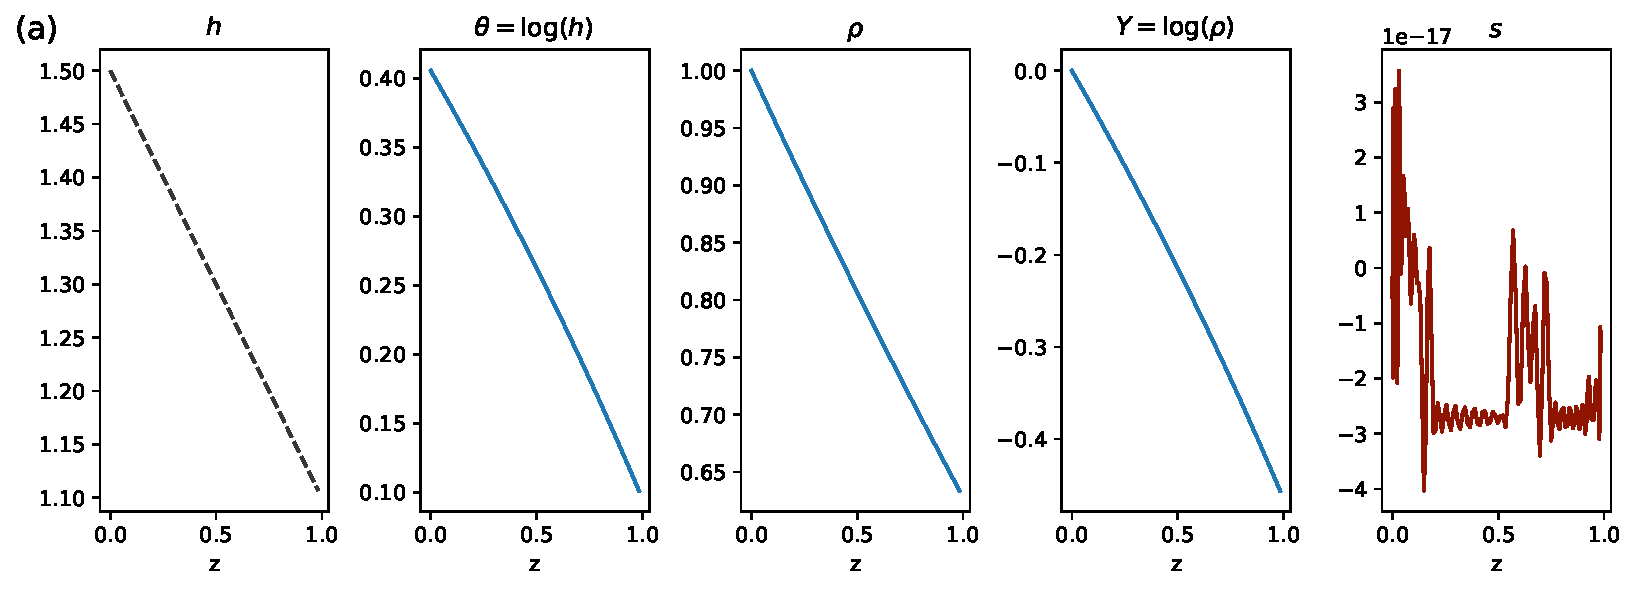
\includegraphics[width=\textwidth,height=6cm]{kramers_initial_condition_linear_nh0.5_eps-2.22e-16_gamma1.67.pdf} \\
    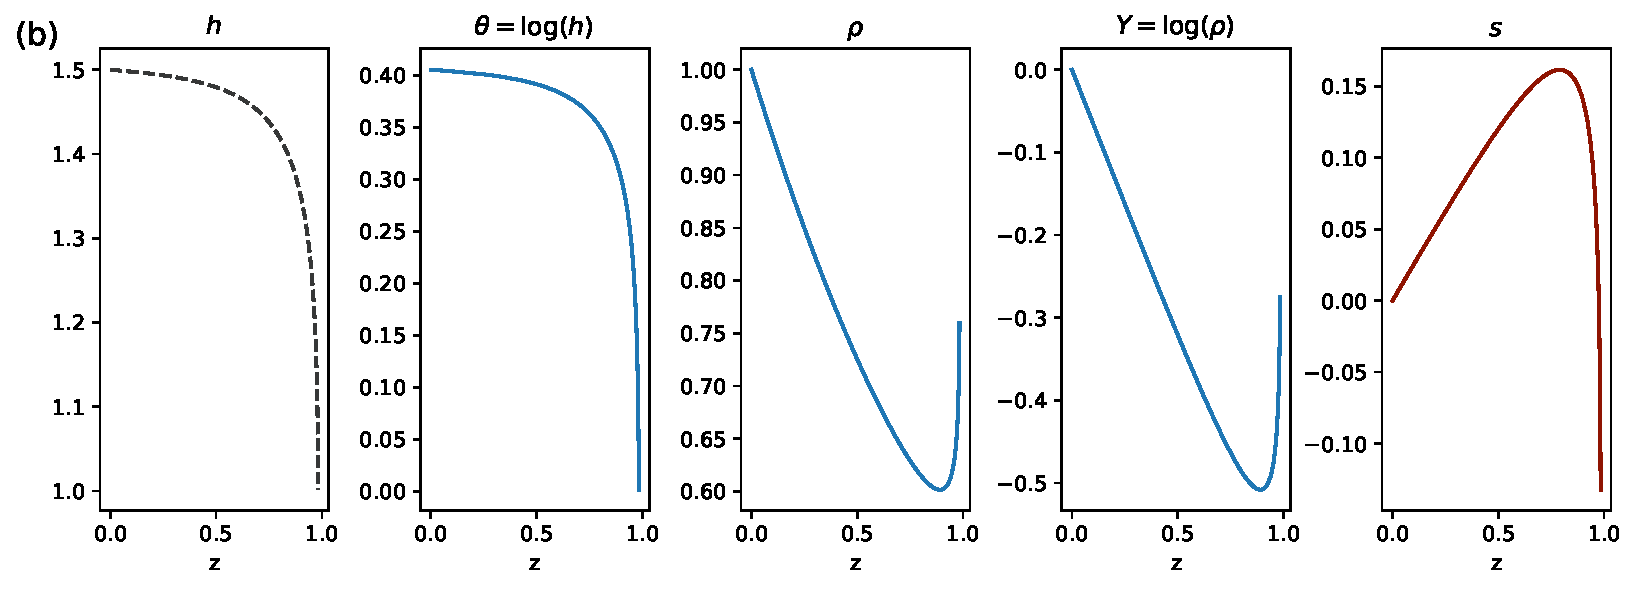
\includegraphics[width=\textwidth,height=6cm]{kramers_solve_h_linear_nh0.5_eps-2.22e-16_gamma1.67.pdf}
    \caption{(a) Initial condition given to the hydrostatic equations. (a) Hydrostatic equilibrium solutions using the first formalism. Here the boundary conditions are $h(z=0)=h_{bot}=1.5,~h(z=L_{z})=1.0,~\theta(z=0)=0$.}
    \label{fig:first_figure}
\end{figure}

Figure \ref{fig:first_figure} shows the (a) initial conditions and the (b) solution from the first formalism (enthalpy). With the sharp drop in entropy near the top boundary, it is likely that the system will be convection. However, the solutions aren't polytropic. The second formalism doesn't converge. (It is the jump in the upper boundary condition that creates an issue.)


Furthermore, Figure \ref{fig:second_figure} shows (a) the initial conditions, and the solutions from both (a) first (enthalpy) and (b) second (log enthalpy) formalism. The initial conditions, in this case, are constant. With the boundary condition set to mismatch at the top boundary, the first formalism does lead to polytrope-like solutions but are convectively stable. 

\begin{figure}
    \centering
    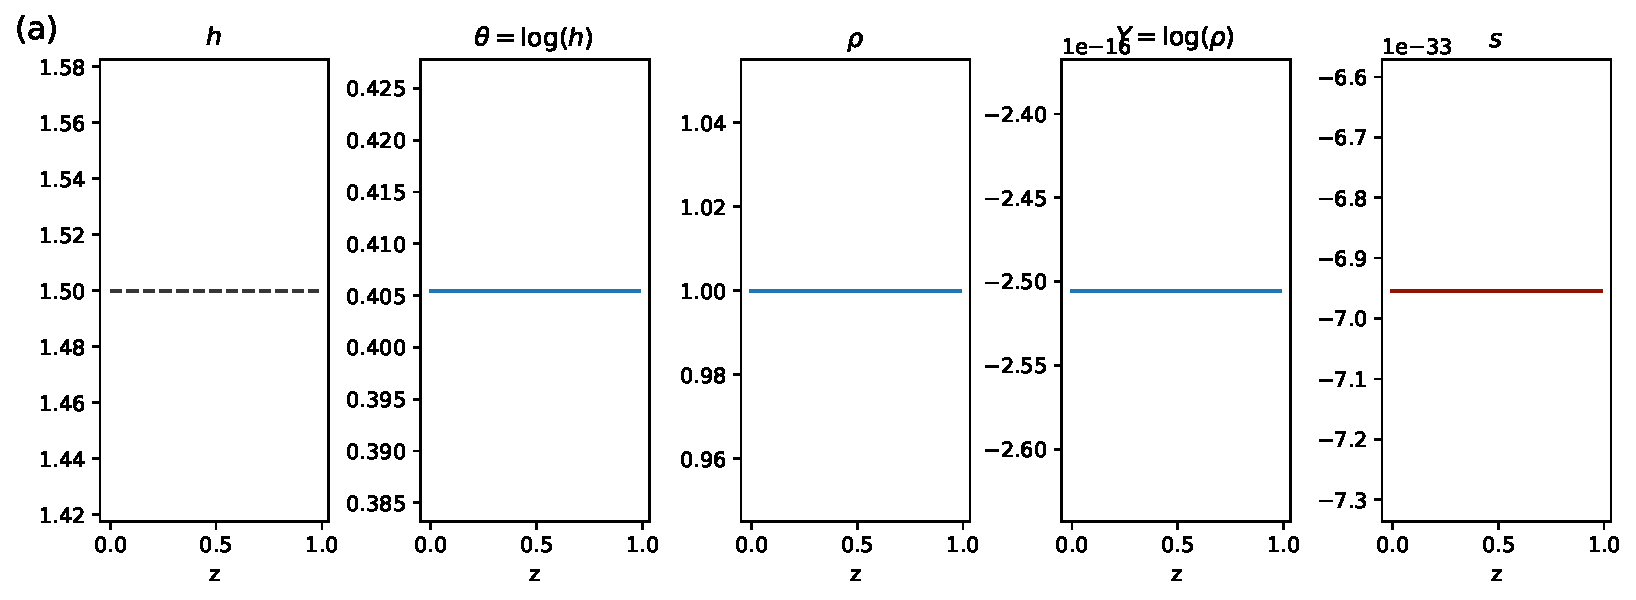
\includegraphics[width=\textwidth,height=6cm]{kramers_initial_condition_linear_ic1_nh0.5_eps-2.22e-16_gamma1.67.pdf}\\
    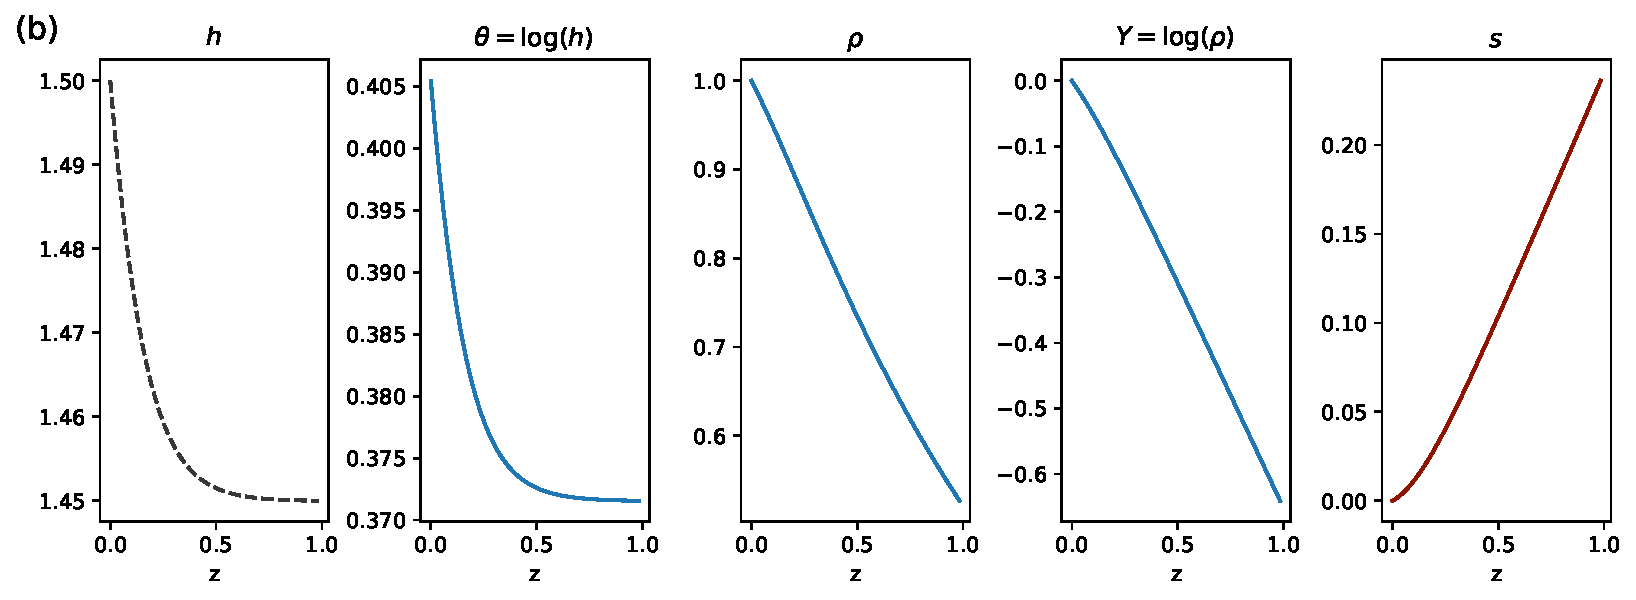
\includegraphics[width=\textwidth,height=6cm]{kramers_solve_h_linear_ic1_nh0.5_eps-2.22e-16_gamma1.67.pdf}\\
    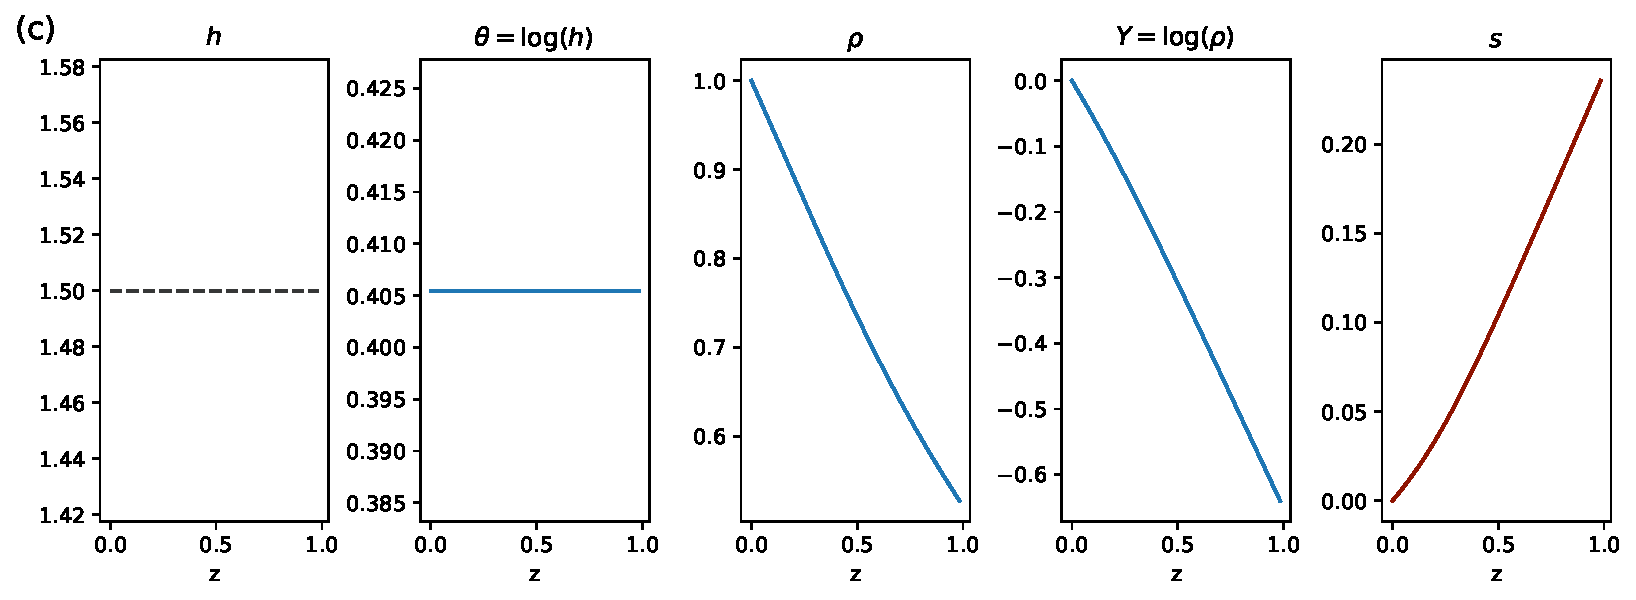
\includegraphics[width=\textwidth,height=6cm]{kramers_solve_theta_linear_ic1__nh0.5_eps-2.22e-16_gamma1.67.pdf}
    \caption{Same as Figure 1 but with boundary conditions for (b) $h(z=0)=h_{bot}=1.5,~h(z=L_{z}=1.45),~Y(z=0)=0$, and for (c) $\theta(z=0)=\log(h_{bot})=\log(1.5),~\theta(z=L_{z})=\log(1.45),~Y(z=0)=0$.}
    \label{fig:second_figure}
\end{figure}





\end{document}